\documentclass{ximera}
% \usepackage{tikz}
% \usepackage{pgfplots}
% ../preamble.tex
% \addPrintStyle{..}

\begin{document}
    \title{TikZ: height issue}
    \begin{abstract}\end{abstract}
    \maketitle


START
 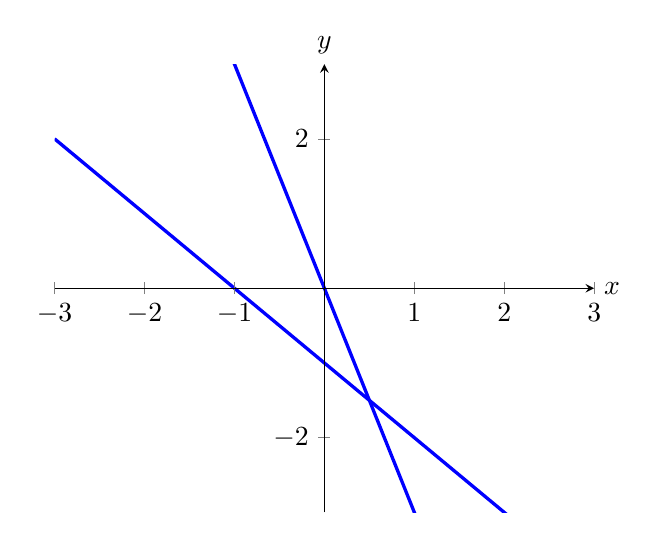
\begin{tikzpicture}
      \begin{axis}[
          xmin=-3, xmax=3,ymin=-3,ymax=3,domain=-3:3,
          %view={0}{90},
          axis lines =center, xlabel=$x$, ylabel=$y$,
          every axis y label/.style={at=(current axis.above origin),anchor=south},
          every axis x label/.style={at=(current axis.right of origin),anchor=west},
          axis on top,
        ]
        \addplot[blue,very thick]{-3*x};
        \addplot[blue,very thick]{-x-1};
    \end{axis}
    \end{tikzpicture}
END


START
 \begin{tikzpicture}
      \begin{axis}[
          xmin=-3, xmax=3,ymin=-3,ymax=3,domain=-3:2,
          %view={0}{90},
          axis lines =center, xlabel=$x$, ylabel=$y$,
          every axis y label/.style={at=(current axis.above origin),anchor=south},
          every axis x label/.style={at=(current axis.right of origin),anchor=west},
          axis on top,
        ]
        \addplot[blue,very thick]{-3*e^x};
        \addplot[blue,very thick]{-x-1};
    \end{axis}
    \end{tikzpicture}
END

\end{document}